\section{Билет 24. Интегральные операторы с непрерывными и полярными ядрами в ограниченной области, их непрерывность в пространстве $C(\bar G)$. Приближение операторов с полярными ядрами операторами с непрерывными ядрами.}
% Затехал: Игорь Молибог
 
\begin{definition}[Интегральное уравнение Фредгольма второго рода]
Уравнение вида $$u(x) = \lambda \int_{G}K(x,y)u(y)dy + f(x)$$ называется интегральным уравнением Фредгольма 2-го рода.

Здесь:
\begin{itemize}
\item $x \in \bar G$, $G$ --- ограниченная область в $\R^3$;
\item $f(x) \in C(\bar G)$ --- задана;
\item $K(x, y): (\bar G \times \bar G) \to \R$.
\item $\lambda$ --- числовой параметр;
\item $u(x) \in C(\bar G)$ --- искомая функция.
\end{itemize} 
\end{definition}

\begin{definition}[Интегральный оператор]
Оператор $K$ такой, что $$(Ku)(x) = \int_{G}K(x,y)u(y)dy,$$ называется интегральным оператором с ядром $K(x,y).$
\end{definition}

\begin{theorem}
Если ядро $K(x,y) \in C(\bar G \times \bar G),$ то оператор $K$ ограничен в $C(\bar G)$ и имеет место оценка $$\|K\| \le \max_{x\in G}\int_G|K(x,y)|dy \le \max_{x,y \in \bar G}|K(x,y)|mes G$$

\end{theorem}

\begin{proof}

Если $K(x,y)\in C(\bar G \times \bar G),$ то $K:C(G) \to C(G)$.

$\|Ku\|_{C(\bar G)} = \max\limits_{\bar G} |(Ku)(x)| = \max\limits_{\bar G} |\int_G K(x,y)u(y)dy| \le  \max\limits_{\bar G} \int_G |K(x,y)||u(y)|dy \le \max_{x \in \bar G} \max\limits_{y \in \bar G} |u(y)|\int_G|K(x,y)|dy = \|u\|_{C(\bar G)}\max\limits_{x \in \bar G}\int_G|K(x,y)|dy \Rightarrow \|K\| = \sup\limits_{\|u\|_{C(\bar G)}=1}\frac{\|Ku\|_{C(\bar G)}}{\|u\|_{C(\bar G)}} \le \max_{x \in \bar G}\int_G |K(x,y)|dy$

\end{proof}


\begin{definition}[Полярное ядро]
Ядро $K(x,y)$ называется полярным, если его можно представить в виде $K(x,y) = \frac{\kappa(x,y)}{|x-y|^\alpha} \Forall x,y \in \bar G,\ x\ne y,$ где $\kappa \in C(\bar G \times \bar G),$ $\alpha < n$ --- размерность пространства.
\end{definition}

\begin{lemma}[Признак полярного ядра]
Ядро $K$ является полярным $\Leftrightarrow K(x,y) \in C((\bar G \times \bar G)\backslash\{x=y\})$ и $|K(x,y)| \le \frac{B}{|x-y|^\beta} \Forall x, y \in \bar G, x \ne y, B>0, \beta < n.$
\end{lemma}

\begin{proof}
($\Rightarrow$): Пусть ядро полярное. Тогда $\exists B: |\kappa| \le B$ на $\bar G \times \bar G$ и $|K| \le \frac{B}{|x-y|^\alpha}.$
\\
($\Leftarrow$): Пусть $\beta < n \Rightarrow \Exists \eps > 0: \beta+\eps < n.$ Рассмотрим $\kappa =  \begin{cases}
   K(x,y)|x-y|^{\beta+\eps}, &x,y\in G, x\ne y;\\
   0, & x=y\in G.
 \end{cases}
$

Построенная $\kappa$ непрерывна в $(\bar G \times \bar G)\backslash\{x=y\}.$

Возьмем $x^0,y^0 \in G, x^0 \ne y^0:$
$|\kappa(x,y) - \kappa(x^0, x^0)| = |\kappa(x,y)| \le |K||x-y|^{\beta+\eps} \le \frac{B}{|x-y|^\beta}|x-y|^{\beta+\eps}\le B|x-y|^\eps = B|(x-x^0)-(y-y^0)|^\eps \le B(|x-x^0|+|y-y^0|)^\eps \Rightarrow \kappa$ непрерывна всюду в $\bar G \times \bar G.$

Очевидно из определения $\kappa,$ что можем записать $K(x,y) = \frac{\kappa(x,y)}{|x-y|^{\beta+\eps}},$ т.е. это ядро -- полярное по определению.
\end{proof}


\begin{definition}[Транспонированное ядро]
Ядром, транспонированным к ядру $K(x,y),$ называется ядро $K'(x,y) = K(y,x).$ Соответствующий оператор $K'$ так же называют транспонированным.
\end{definition}

\begin{theorem}
Интегральный оператор $K$ с полярным ядром является ограниченным оператором в $C(\bar G).$ Справедлива оценка: $\|K\| \le \sup_{x\in G}\int_G|K(x,y)|dy.$ $\Forall \eps > 0$ оператор $K$ можно представить в виде суммы $K = K_\eps^{cont}+K_\eps^{pol},$ где $\|K_\eps^{pol}\| \le \eps,$ $\|(K_\eps^{pol})'\| \le \eps,$ $K_\eps^{cont}$ --- и.о. с непрерывным ядром, $K_\eps^{pol}$ --- и.о. с полярным ядром.
\end{theorem}

\begin{proof} $\ $
\begin{enumerate}
\item{
Пусть $\psi(y) = K(x,y)u(y).$ Функция $\psi$ непрерывна при $y \ne x.$

В особенности: $|\psi(y)| = |K(x,y)||u(y)| \le \frac{B}{|x-y|^\alpha} \|u\|_{C(\bar G)}$ -- интегрируема, т.к. $\alpha < n.$

Значит, порождается функция $\phi(x) = \int_G\psi(y)dy = \int_G K(x,y)u(y)dy$ --- этот интеграл существует $\forall x \in \bar G.$
}

\item{Определим $\delta-$срезку функции $\frac{1}{|x-y|^\alpha}:$ $$\left(\frac{1}{|x-y|^\alpha}\right)_\delta = \begin{cases}
   \frac{1}{|x-y|^\alpha}, &|x-y|\ge \delta;\\
   \frac{1}{\delta^\alpha}, & |x-y|<\delta.
 \end{cases} \in C (\R^n \times \R^n)$$
}
\begin{center}
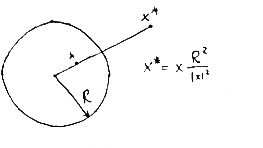
\includegraphics[width=0.2\textwidth]{24_1_new}
\end{center}

\item{Представим $K(x,y) = K^1_\delta (x,y) + K^2_\delta(x,y),$ где $K^1_\delta (x,y) = \kappa(x,y)(\frac{1}{|x-y|^\alpha})_\delta,$ $$K^2_\delta(x,y) = \begin{cases}
   0, &|x-y|\ge \delta;\\
   \kappa(x,y)(\frac{1}{|x-y|^\alpha}-\frac{1}{\delta^\alpha}), & |x-y|<\delta.
 \end{cases}$$
}

\item{ Выберем произвольно $u(x) \in C(\bar G)$ и рассмотрим $\|K^2_\delta u\|_{C(\bar G)}$: 

$\|K^2_\delta u\| = \max_{x \in G} |\int_{|y-x|<\delta}\kappa(x,y)(\frac{1}{|x-y|^\alpha}-\frac{1}{\delta^\alpha})u(y)dy| \le B\|u\|_{C(\bar G)}\int_{|y-x|<\delta}\frac{dy}{|x-y|^\alpha} = B \|u\|_{C(\bar G)}\int_{|z|<\delta}\frac{dz}{|z|^\alpha}.
$

Замена $\begin{cases}
   x_k = r\sin\phi_1...\sin\phi_{k-1}\cos\phi_k, &k = 1, \dots, n-1;\\
   x_n = r\sin\phi_1...\sin\phi_{n-1},
 \end{cases}$ где $\phi_k \in [0, \Pi], \phi_n \in [0, 2\Pi]$
 
Якобиан $J = \frac{D(x_1, \dots, x_n)}{D(r, \phi_1, \dots, \phi_{n-1})} = r^{n-1}\sin^{n-2}\phi_1\sin^{n-3}\phi_2\dots\sin\phi_{n-1}.$ Получили:

$$\|K^2_\delta a\| \le C_1\|u\|_{C(G)}\int_0^\delta\frac{r^{n-1}}{r^\alpha}dr = C\|u\|_{C(G)}\delta^{n-\alpha} \to 0 \text{ при } \delta \to 0.$$

Получили $K^2_\delta u \to Ku$ по норме $\Rightarrow Ku \in C(\bar G).$
 
}

\item{$\|K\| \le \|K^1_\delta\| + \|K^2_\delta\|\le C\delta^{n-\alpha} + \|K^1_\delta\| < \infty$ $\Rightarrow K$ --- ограничен.

Для транспонированного ядра все рассуждения аналогичны, т.к. полярное ядро $K = \frac{\kappa(x,y)}{|x-y|^\alpha}$ при замене $x$ на $y$ изменяет только непрерывный числитель $\kappa$.
}

\end{enumerate}
\end{proof}










